\documentclass{article}
\usepackage[utf8]{inputenc}

\title{Relatório Web Semântica \\ \textbf{Domínio}: Agricultura}
\author{Romário Ferreira}
\date{Quinta-feira, 31 de outubro de 2019}

\usepackage{natbib}
\usepackage{graphicx}

\begin{document}

\maketitle

\section{Introdução}
Este relatório tem como intuito relatar o assunto estudado na logica descritiva e a implementação 
de um domínio com caso de estudo. O objetivo deste relatório é mostrar como ocorreu a solução do problema em estudo e bem como apresentar os resultados obtidos ao aplicar o problema no software 
\textit{protegé}, assim sendo adotou-se o domínio para estudo como sendo Agricultura, pois bem, procurou-se escolher este domínio pois ele é conhecido e de fácil entendimento para os demais, e também ao realizar a modelagem da lógica descritiva não ocorrerem problemas de desconhecimento do domínio.

Para implementação do domínio e representar a forma do conhecimento, utilizou-se o software como alidado para realizar as inferências lógicas, neste contexto inseriu-se no software o Tbox e Abox,


Neste relatório abordou-se o estudo do domínio agricultural, desta forma aplicado a utilizando logica descritiva, permitindo-se a contrução do tbox e abox, assim pode-se aplicar ao software protégé para melhor entendimento.


\section{Desenvolvimento}
    Para dar inicio ao estudo definimos o domínio como sendo Órgão público em especifico IBAMA, porém notamos dificuldades neste domínio e decidimos alterar-lo, assim sendo escolhemos outro domínio
    no qual é voltado a Agricultura, posteriormente decidimos realizar o tbox, assim observou-se o 
    domínio para coletar as informações necessárias para realização do mesmo.
    
    \begin{table}[!ht]
        \centering
        \begin{tabular}{c|c|c|c}
            Clima   &   Solo    &  Agricultor & Temperatura \\
            \hline
            Período &  Agrotóxico & Semente  & Praga  \\
        \end{tabular}
        \caption{Conceitos}
        \label{tab:my_label}
    \end{table}
    
    \begin{table}[!ht]
        \centering
        \begin{tabular}{c|c|c}
            Colher&Plantar&Adubar\\
            \hline
            Aplicar&Tem&Possui\\
        \end{tabular}
        \caption{Relações}
        \label{tab:my_label}
    \end{table}
    
    
    \section{Inferências Obtidas com }
   
        \begin{figure}[!ht]
            \centering % para centralizarmos a figura
            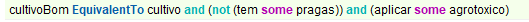
\includegraphics[width=1\textwidth]{imagens/inferencia/inf_01.PNG} % leia abaixo
            \caption{Apresenta a ocorrencia da disjunção entre agricultor e pragas}
            \label{figura:disjunt}
        \end{figure}
        \begin{figure}[!htp]
            \centering % para centralizarmos a figura
            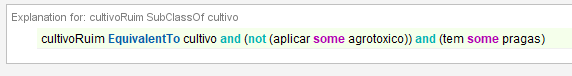
\includegraphics[width=1\textwidth]{imagens/inferencia/inf_02.PNG} % leia abaixo
            \caption{Apresenta a ocorrencia da disjunção entre agricultor e pragas}
            \label{figura:disjunt}
        \end{figure}
        \begin{figure}[!htp]
            \centering % para centralizarmos a figura
            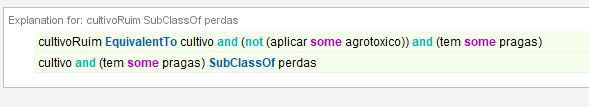
\includegraphics[width=1\textwidth]{imagens/inferencia/inf_03.PNG} % leia abaixo
            \caption{Apresenta a ocorrencia da disjunção entre agricultor e pragas}
            \label{figura:disjunt}
        \end{figure}
        \begin{figure}[!htp]
            \centering % para centralizarmos a figura
            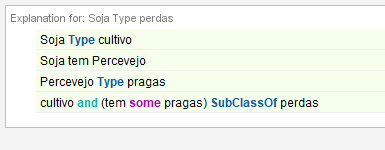
\includegraphics[width=1\textwidth]{imagens/inferencia/inf_04_soja.PNG} % leia abaixo
            \caption{Apresenta a ocorrencia da disjunção entre agricultor e pragas}
            \label{figura:disjunt}
        \end{figure}
    
 
% Texto original
%%Dois ou mais conjuntos são seprardos entre si, mas ao realizar uma 
%%disjunção os conjuntos além de serem separados são também diferentes 
%%entre sí, neste caso apresentado na imagem Agricultor e pragas são 
%%disjuntos entre.

Foi possível verificar em dois conjuntos suas diferenças, ao realizar-mos uma 
disjunção dos conjuntos, notamos que além de serem serparados, são diferentes entre
si, neste caso apresentamos a imagem com conjunto agricultor e pragas os quais 
são disjuntos.


\begin{figure}[!htp]
    \centering % para centralizarmos a figura
    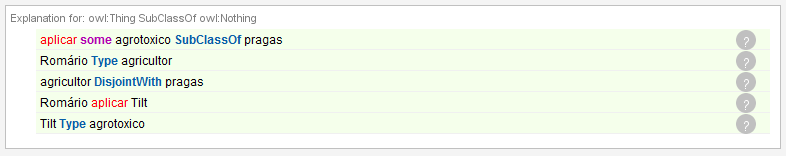
\includegraphics[width=1\textwidth]{imagens/disjunt.png} % leia abaixo
    \caption{Apresenta a ocorrencia da disjunção entre agricultor e pragas}
    \label{figura:disjunt}
\end{figure}

\section{Conclusão}
``I always thought something was fundamentally wrong with the universe'' \citep{adams1995hitchhiker}

\bibliographystyle{plain}
\bibliography{references}
\end{document}
